% !TeX spellcheck = en_US
% !TeX root = notes.tex
\section{Quiz 1}

\subsection{Question 1}
Rosie is considering starting a clothing stall at a weekend market in her suburb. Which of the following statements is true? (Single Answer)
\begin{enumerate}
	\item \hl{Rosie can use economic thinking to determine the selling price of her cloths}
	\item Rosie should only use economics in this situation and not accounting
	\item Clothing is not a scarce resource
	\item Rosie cannot use economics because her business is too small
	\item Rosie does not have to make trade-offs in this situation
\end{enumerate}

\subsection{Question 2}
Andy is a baker in Brisbane. It costs him \$0.50 to produce each loaf of bread. Andy can sell 10 loaves of bread for \$40 and 11 loaves of bread for \$43. Which of the following statements are true: (Multiple Answers)
\begin{enumerate}
	\item \hl{The marginal cost of producing a loaf of bread is \$0.50}
	\item \hl{Andy should produce the eleventh loaf of bread because marginal benefit is greater than the average cost}
	\item There is insufficient information to determine the marginal benefit of producing the eleventh loaf of bread
	\item \hl{The marginal benefit of producing the eleventh loaf of bread is \$3}
\end{enumerate}\vspace{1em}
Working:
\begin{table}[H]
	\centering
	\begin{tabular}{r|rr}
		Number of Loaves & Money Gained & Total Benefit\\\hline
		10 & \$40 & \$35\\
		11 & \$43 & \$37.5\\
	\end{tabular}
\end{table}
\noindent Average cost: \$0.50\\
Marginal Benefit of 11th bread: \$3

\subsection{Question 3}
Jeremy is considering whether to go to the beach on the weekend. His alternatives, in order of preference from most to least preferred, are:
\begin{enumerate}
	\item Visiting his family
	\item Studying for a test
	\item Working at his casual job for 5 hours with a wage of \$15/hour
\end{enumerate}
Select the item from the list provided to make the following statements true:\\\\
Average Cost; The net benefit of working at his casual job; should not; visiting his family; 5 hours; working at his casual job; should; studying for a test; the net benefit of studying for a test; marginal benefit; marginal cost; \$15/hour.\\\\
In considering whether to go to the beach, the value of casual work foregone \_\_\_\_\_\_\_\_\_\_ be included in a marginal analysis. The opportunity cost of going to the beach is \_\_\_\_\_\_\_\_\_\_. If going to the beach suddenly is \textbf{not} an option for Jeremy, then \_\_\_\_\_\_\_\_\_\_ is the opportunity cost of visiting his family.\\\\
Answer: Should not; visiting his family; studying for a test

\subsection{Question 4}
Lillian bought a limited edition ``Harry Potter'' costume at an exclusive fan event. She can now either:
\begin{enumerate}
	\item Sell the costume on eBay for \$534
	\item Keep the costume for per personal use
\end{enumerate}
If she sells the costume on eBay she will have to pay \$10 to ship it to the customer. If she keeps the costume she expects to gain \$651 of enjoyment and will need to spend \$88 on maintenance and cleaning. When comparing the net benefits of selling the costume minus the net benefits of keeping it, what is the economic surplus/loss? Answer to the nearest whole number.\\\\
Answer:
Let $x$ be the benefit of selling. Let $y$ be the benefit of keeping. Let $t$ be the economic surplus/loss of selling minus keeping
\begin{align*}
	x &= \$534 - \$10\\
	&= \$524\\
	y &= \$651 - \$88\\
	&= \$563\\
	t &= x - y\\
	&= \$524 - \$563\\
	&= -\$39
\end{align*}

\subsection{Question 5}
Lucy pays \$40 to enter a theme park. When inside the park, Lucy considers how many rides she should have on the ``Big Drop''. She expects to gain an incremental benefit of \$25 of enjoyment from the first ride, then gain subsequent incremental benefits of \$20 from the second, \$15 from the third, \$10 from the fourth and \$5 from the fifth. The cost of each ride is \$15.\\\\
In determining how many rides to have, the entry free is a/an \_\_\_\_\_\_\_\_\_\_ cost. Using marginal analysis, Lucy should have how many rides? \_\_\_\_\_\_\_\_\_\_. The maximum surplus for Lucy, from doing the number of rides you found in part b, is \$\_\_\_\_\_\_\_\_\_\_. Answer to nearest whole number.\\\\
\begin{table}[H]
	\centering
	\begin{tabular}{rrr}
		Ride No & Benefit & Benefit - Cost\\\hline
		1 & \$25 & \$10\\
		2 & \$20 & \$5\\
		3 & \$15 & \$0\\
		4 & \$10 & -\$5\\
		5 & \$5 & -\$10
	\end{tabular}
\end{table}
Answer: Sunk Cost; 2 rides; \$15

\subsection{Question 6}
Seth and Ryan are roommates, living together in a house. Both roommates are currently considering who should cook dinner and who should clean up afterwards. Ryan was a trainee chef and a skilled cook. Seth, on the other hand, had previously only lived at home, where his mum cooked everything for him. However, Seth had become very efficient at cleaning up after meals and packing things away. Which of the following is true: (Multiple Answers)
\begin{enumerate}
	\item Seth has a comparative advantage in cooking dinner
	\item \hl{Thinking like an economist in this situation, the roommates should specialise with Ryan cooking and Seth cleaning}
	\item Ryan has a lower opportunity cost for cooking dinner
\end{enumerate}

\subsection{Question 7}
Lily and May operate a store that sells fresh juices. There are two main activities: cutting the fruit and juicing the fruit. Lily and May are deciding who should cut and who should juice in order to maximize output.
\begin{table}[H]
	\centering
	\begin{tabular}{r|c|c}
		& Cutting (kg/hr) & Juicing (kg/hr)\\\Xhline{1pt}
		Lily & 3 & 5\\\hline
		May & 2 & 8
	\end{tabular}
\end{table}
Which of the following statements are true: (Multiple Answers)
\begin{enumerate}
	\item For Lily, the opportunity cost of 1kg of cutting is 1.2kg of juicing
	\item \hl{For May, the opportunity cost of 1kg of juicing is 0.25kg of cutting}
	\item May should specialize in cutting
	\item Lily has an absolute advantage in juicing
\end{enumerate}
\begin{table}[H]
	\centering
	\begin{tabular}{r|c|c}
		& Cutting (kg/hr) & Juicing (kg/hr)\\\Xhline{1pt}
		Lily & $\frac{3}{3}=1$ & $\frac{5}{3}=1.67$\\\hline
		May & $\frac{2}{2}=1$ & $\frac{8}{2}=4$
	\end{tabular}
\end{table}
\begin{table}[H]
	\centering
	\begin{tabular}{r|c|c}
		& Cutting (kg/hr) & Juicing (kg/hr)\\\Xhline{1pt}
		Lily & $\frac{3}{5}=0.6$ & $\frac{5}{5}=1$\\\hline
		May & $\frac{2}{8}=0.25$ & $\frac{8}{8}=1$
	\end{tabular}
\end{table}

\subsection{Question 8}
Australia's second biggest tading partner is Japan. Among other things, Australia exports coal to Japan while importing cars. In one trading day, Japan can produce 12 cars per hour and Australia can produce a total of 80 tonnes of coal per hour. Assume cars and coal are the only two things that the two countries trade. Also assume one trading day is 9 hours long.\\
Select the item from the list provided to make the following statements true.\\\\
Cars per hour; 81; Opportunity cost; 720 tonnes of coal; Comparative advantage; 96; Minimized; 108; Cars; Absolute advantage; Tonnes of coal; Maximized\\\\
By specializing, the two countries have minimized \_\_\_\_\_\_\_\_\_\_. In one trading day, Australia will produce \_\_\_\_\_\_\_\_\_\_. In one trading day, Japan will produce \_\_\_\_\_\_\_\_\_\_ cars.\\\\
Answer: Opportunity Cost; 720 tonnes of coal; 108;

\subsection{Question 9}
Lise is hosting a party in 6 hours' time. She wishes to provide guests with her homemade dips -- guacamole and hummus. Shown below is Lisa's production possibilities curve for the next 6 hours.
\begin{figure}[H]
	\centering
	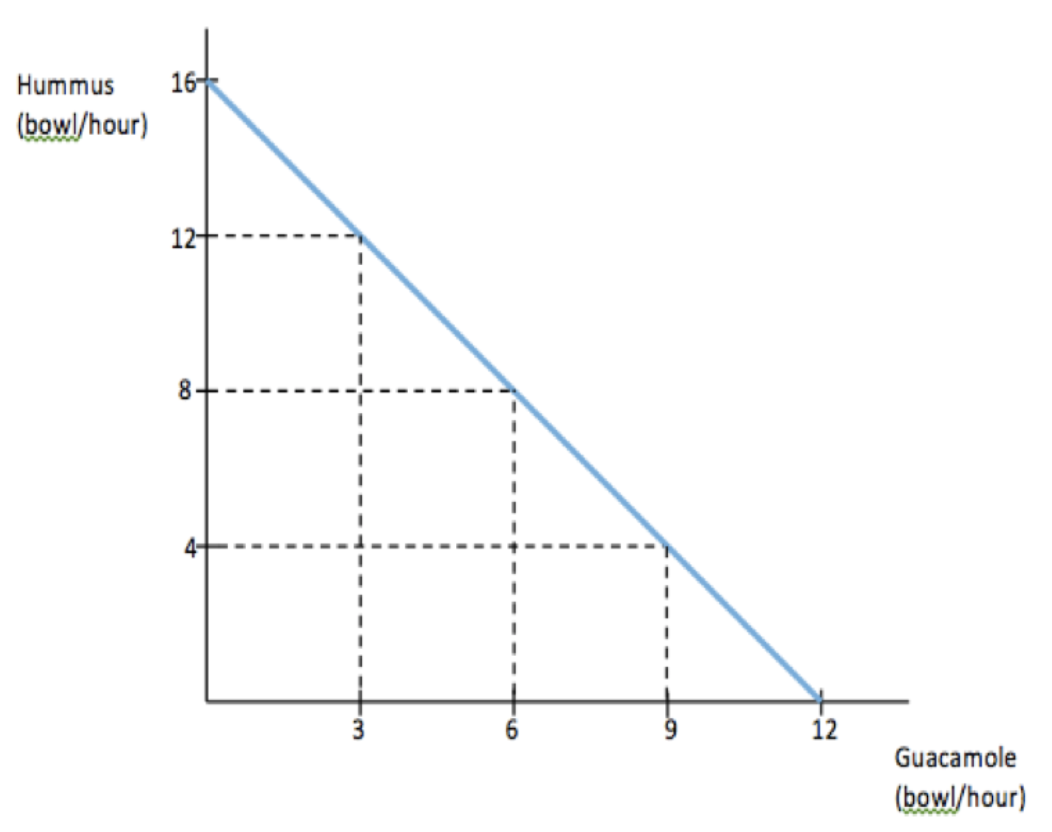
\includegraphics[width=0.5\linewidth]{cml_1_9}
\end{figure}
\noindent What is Lisa's opportunity cost of producing 1 bowl of guacamole? Answer to the nearest two decimal places. In bowls of hummus.\\\\
Answer:
\begin{align*}
	y &= mx+c\\
	16 &= 0m+c\tag{Sub when $x$ is zero}\\
	c &= 16\\
	\therefore y &= mx + 16\\
	0 &= 12m + 16\tag{Sub when $y$ is zero}\\
	-16 &= 12m\\
	m &= \frac{-16}{12} = \frac{-8}{6} = \frac{-4}{3}\\
	\therefore y &= 16 - \frac{4}{3}x\\
	y&= 16 - \frac{4}{3}\times1\tag{Produce 1 bowl of guacamole}\\
	y &= 14.67
\end{align*}
Therefore the opportunity cost of producing 1 bowl of guacamole is $16 - 14.67 = 1.33$ bowls of hummus.

\subsection{Question 10}
Martha is a florist who is trying to maximize her output. She can produce two types of flowers: lilies and violets. Shown below is Martha's production possibilities curve. The X denotes the quantity of each flower she is currently producing.
\begin{figure}[H]
	\centering
	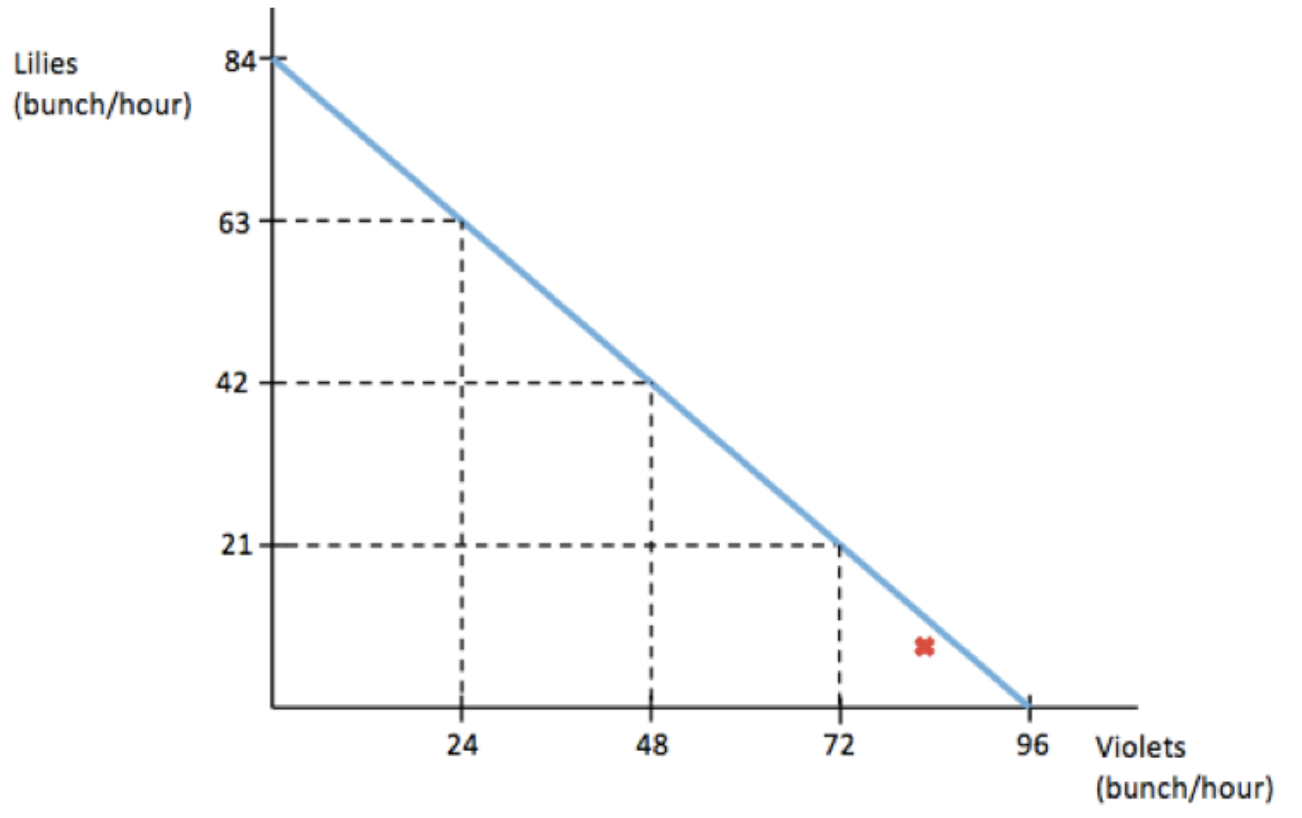
\includegraphics[width=0.5\linewidth]{cml_1_10}
\end{figure}
\noindent Answer the following questions:
\begin{itemize}
	\item Is the current output attainable? (\hl{Yes}/No)
	\item Calculate the opportunity cost of producing 1 bunch of lilies. Answer to the nearest two decimal places. \_\_\_\_\_\_\_\_\_\_ bunches of violets
	\item Is the current output efficient, \hl{inefficient} or neither because it is unattainable?
\end{itemize}\vspace{1em}
\begin{align*}
	y &= 84 - \frac{21}{24}x\\
	1 &= 84 - \frac{21}{24}x\tag{Producing 1 bunch of lillies}\\
	\frac{21}{24}x &= 83\\
	x &= \frac{83\times24}{21}\\
	x &= 94.86
\end{align*}
Therefore the opportunity cost of producing 1 bunch of lilies is $96 - 94.86 = 1.14$